\documentclass{article}
\usepackage{a4wide}
\usepackage[utf8]{inputenc}
\usepackage{amsmath}
\usepackage{mathtools}
\usepackage{amssymb}
\usepackage[english]{babel}
\usepackage{mdframed}
\usepackage{systeme,}
\usepackage{lipsum}
\usepackage{relsize}
\usepackage{caption}
\usepackage{tikz}
\usepackage{tikz-3dplot}
\usepackage{pgfplots}
\usepackage{harpoon}%
\usepackage{graphicx}
\usepackage{wrapfig}
\usepackage{subcaption}
\usepackage{authblk}
\usepackage{float}
\usepackage{listings}
\usepackage{xcolor}
\usepackage{amsmath}
\usepackage{chngcntr}
\usepackage{amsthm}
\usepackage{comment}
\usepackage{commath}
\usepackage{hyperref}%Might remove, adds link to each reference
\usepackage{url}
\newcommand{\w}{\omega}
\newcommand{\curl}[1]{\mathbf{\nabla}\times \mathbf{#1}}
\newcommand{\grad}{\mathbf{\nabla}}
\newcommand{\dive}[1]{\mathbf{\nabla}\cdot \mathbf{#1}}
%\newcommand{\crr}{\mathfrak{r}}
\usepackage{calligra}
\newcommand{\average}[1]{\langle #1 \rangle}
%\newcommand{\norm_}[1]{|| #1 ||}

\DeclareMathAlphabet{\mathcalligra}{T1}{calligra}{m}{n}
\DeclareFontShape{T1}{calligra}{m}{n}{<->s*[2.2]callig15}{}
\newcommand{\crr}{\mathcalligra{r}\,}
\newcommand{\boldscriptr}{\pmb{\mathcalligra{r}}\,}
\newcommand{\res}[2]{\text{Res}(#1,#2)}

\title{Handin 1}
\author{Author : Andreas Evensen}
\date{Date: \today}
\definecolor{codegreen}{rgb}{0,0.6,0}
\definecolor{codegray}{rgb}{0.5,0.5,0.5}
\definecolor{codepurple}{rgb}{0.58,0,0.82}
\definecolor{backcolour}{rgb}{0.95,0.95,0.92}

\lstdefinestyle{mystyle}{
    backgroundcolor=\color{backcolour},   
    commentstyle=\color{codegreen},
    keywordstyle=\color{magenta},
    numberstyle=\tiny\color{codegray},
    stringstyle=\color{codepurple},
    basicstyle=\ttfamily\footnotesize,
    breakatwhitespace=false,         
    breaklines=true,                 
    captionpos=b,                    
    keepspaces=true,                 
    numbers=left,                    
    numbersep=5pt,                  
    showspaces=false,                
    showstringspaces=false,
    showtabs=false,                  
    tabsize=2
}

\lstset{style=mystyle}

\begin{document}

\maketitle

\section*{1)}
In self-avoiding random walk the mean-square-distance after $N$ step is $\average{R^2} \sim N^{\frac{3}{2}}$. Calculate the pair distribution function $g(r)$.
\subsection*{Solution}
The mean-square-distance after $N$ steps is given by:
The pair distribution function is defined as:
\begin{align*}
    g(r) &= \frac{1}{2\pi r^2}\frac{dn}{dr} = \frac{1}{2\pi r^2}\frac{d}{dr}\left(r^{2}\right)^{2/3}\\
    &= \frac{4}{6\pi}\frac{r^{1/3}}{r^2}.
\end{align*}


\begin{center}
    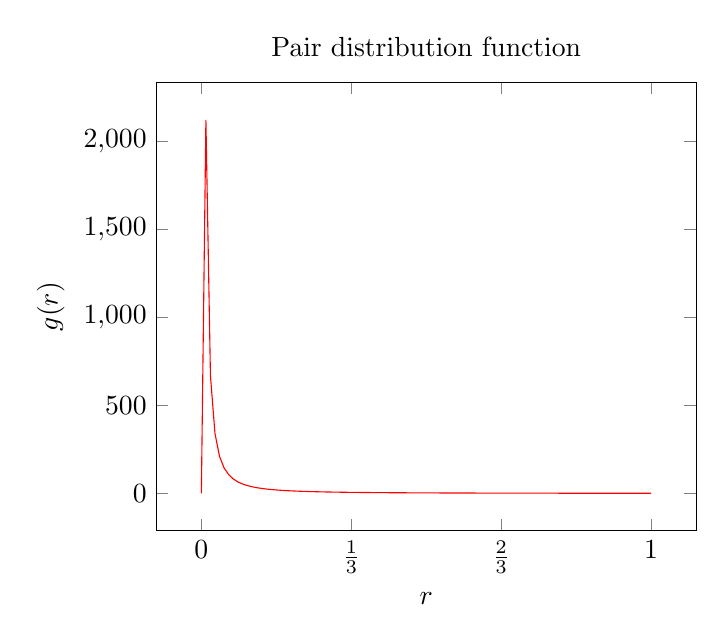
\begin{tikzpicture}
        \begin{axis}[xlabel =$r$,
            ylabel=$g(r)$,
            %axis lines = left,]
            title = {Pair distribution function},
            xtick={0, 1/3, 2/3, 1},
            xticklabels={$0$, $\frac{1}{3}$, $\frac{2}{3}$, $1$},]
            \addplot[domain=0:1, samples=100, color=red]{x^(1/3)/x^2};
        \end{axis}
    \end{tikzpicture}
\end{center}

\section*{2)}
A displacement field is given by the following expression:
\begin{align*}
    u_1 &= \alpha(5x - y + 3z),\\
    u_2 &=\alpha(x+ 8y),\\
    u_3 &=\alpha(-3x+4y+5z).
\end{align*}Where $\alpha$ is small, thereby the assumption of small displacement is satisfied.
Calculate the velocity gradient matrix, decompose it into symmetric and antisymmetric part, find out the three principal directions of strain and the equation for the strain ellipsoid in the frame of its principal axis.
\subsection*{Solution}
\begin{align*}
    \grad{\mathbf{u}} &= \begin{pmatrix}
        \frac{\partial u_1}{\partial x} & \frac{\partial u_1}{\partial y} & \frac{\partial u_1}{\partial z}\\
        \frac{\partial u_2}{\partial x} & \frac{\partial u_2}{\partial y} & \frac{\partial u_2}{\partial z}\\
        \frac{\partial u_3}{\partial x} & \frac{\partial u_3}{\partial y} & \frac{\partial u_3}{\partial z}\\
    \end{pmatrix} = \alpha\begin{pmatrix}
        5 & -1 & 3\\
        1 & 8 & 0\\
        -3 & 4 & 5
    \end{pmatrix}\\
    &=\alpha\underbrace{\begin{pmatrix}
        5&0&0\\
        0&8&2\\
        0&2&5
    \end{pmatrix}}_{\text{Symmetric}} + \underbrace{\alpha\begin{pmatrix}
        0&-1&3\\
        1&0&-2\\
        -3&2&0
    \end{pmatrix}}_{\text{Anti-symmetric}}
\end{align*}In order to find the principal directions of the strain one diagonalizes the symmetric part of the velocity gradient matrix:
\begin{align*}
    \text{det}\left(\mathbf{S} - \lambda\mathbf{I}\right)&=\begin{vmatrix}
        5-\lambda&0&0\\
        0&8-\lambda&2\\
        0&2&5-\lambda
    \end{vmatrix}\\
    &= (5-\lambda)\left((8-\lambda)(5-\lambda) - 4\right)\implies \lambda_i = \{9, 5, 4\}.
\end{align*}One now note that $\text{Trace}(\mathbf{A}) = \sum_i\lambda_i = 18$. \textit{Note}: one has so far not included the constant $\alpha$ however, the eigenvalues of $\alpha\cdot\mathbf{S}$ are equal to the eigenvalues found prior multiplied by $\alpha$.
The eigenvectors and thus the principal directions of the strain are given by:
\begin{align*}
    \mathbf{x_1} = \begin{pmatrix}
        0\\
        2\\
        1
    \end{pmatrix},\quad \mathbf{x_2} = \begin{pmatrix}
        1\\
        0\\
        0
    \end{pmatrix},\quad \mathbf{x_3} = \begin{pmatrix}
        0\\
        -1\\
        2
    \end{pmatrix}.
\end{align*}To find the equation for the strain ellipsoid in the frame of its principal axis we use the following expression:
\begin{comment}
\begin{align*}
    A &= \begin{pmatrix} 
        \frac{\mathbf{x_1}}{\norm{\mathbf{x_1}}}& \frac{\mathbf{x_2}}{\norm{\mathbf{x_2}}} & \frac{\mathbf{x_3}}{\norm{\mathbf{x_3}}}
    \end{pmatrix}
    \cdot\underbrace{\begin{pmatrix}
        9&0&0\\
        0&5&0\\
        0&0&4
    \end{pmatrix}}_{=\mathbf{\Lambda}}\cdot\begin{pmatrix}
        \frac{\mathbf{x_1}}{\norm{\mathbf{x_1}}}& \frac{\mathbf{x_2}}{\norm{\mathbf{x_2}}} & \frac{\mathbf{x_3}}{\norm{\mathbf{x_3}}}
    \end{pmatrix}^{T}\\
    &=\begin{pmatrix} 
        \frac{\mathbf{x_1}}{\sqrt{3}}& \mathbf{x_2} & \frac{\mathbf{x_3}}{\sqrt{3}}
    \end{pmatrix}
    \cdot\begin{pmatrix}
        9&0&0\\
        0&5&0\\
        0&0&4
    \end{pmatrix}\cdot\begin{pmatrix}
        \frac{\mathbf{x_1}}{\sqrt{3}}& \mathbf{x_2} & \frac{\mathbf{x_3}}{\sqrt{3}}
    \end{pmatrix}^{T}\\
    &=\begin{pmatrix}
        0 &5 &0\\
        6\sqrt{3}& 0 &\frac{-4\sqrt{3}}{3}\\
        3\sqrt{3}& 0 &\frac{4\sqrt{3}}{3}
    \end{pmatrix}\cdot\begin{pmatrix}
        \frac{\mathbf{x_1}}{\sqrt{3}}& \mathbf{x_2} & \frac{\mathbf{x_3}}{\sqrt{3}}
    \end{pmatrix}^{T}=\begin{pmatrix}
        5& 0& 0\\
        0& \frac{40}{3}& \frac{10}{3}\\
        0& \frac{14}{3}& \frac{17}{3}
    \end{pmatrix}
    \implies 1&=\frac{1}{3}\left(15x^2+40y^2 + 17z^2 + 24yz\right)
\end{align*}
\end{comment}
The ellipsoid is then given by:
\begin{align*}
    1&=\mathbf{x}^TA\mathbf{x} = \begin{pmatrix}
        x&y&z
    \end{pmatrix}\cdot\mathbf{\Lambda}\cdot\begin{pmatrix}
        x\\
        y\\
        z
    \end{pmatrix}\\
    &=\mathbf{x}^TA\mathbf{x} = \begin{pmatrix}
        x&y&z
    \end{pmatrix}\cdot\alpha\begin{pmatrix}
        5&0&0\\
        0&9&0\\
        0&0&4
    \end{pmatrix}\cdot\begin{pmatrix}
        x\\
        y\\
        z
    \end{pmatrix}\\
    &= \alpha\cdot(5x^2 + 9y^2 + 4z^2)
\end{align*}
\begin{comment}
\begin{center}
    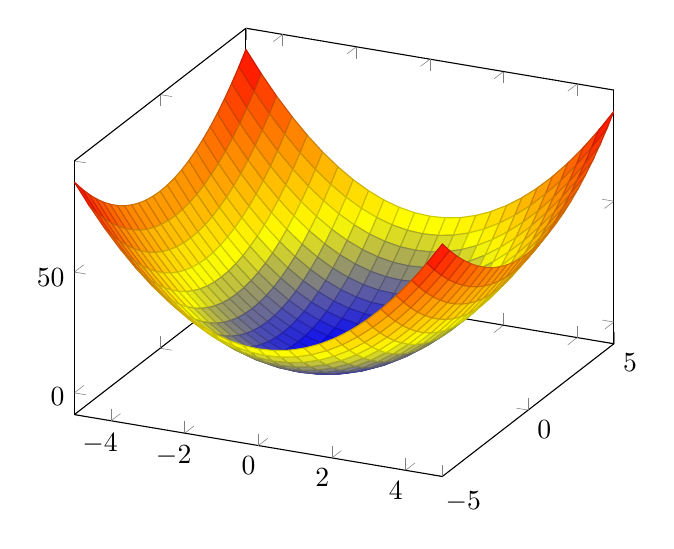
\begin{tikzpicture}
        \begin{axis}
            \addplot3[surf,] {( 9*x^2 + 5*y^2 -1 )*1/4};
        \end{axis}
    \end{tikzpicture}
\end{center}
\end{comment}



\section*{3)}
Show that a small volume change under a general deformation can be expressed as:
\begin{align*}
    \delta V = \oint_S \mathbf{u}\cdot\hat{n}dS.
\end{align*}Where $\hat{n}$ is the outward normal to the surface element $dS$ and $\mathbf{u}$ is the deformation field.
\subsection*{Solution}
Suppose a deformation field: $\mathbf{u}$ of which one wants to calculate the volume change. Suppose a point $\mathbf{r} = (x,y,z)$, then the volume is given by: $dV = dxdydz$.
If the deformation field is small, and the deformation field maps to the point $\mathbf{r}$ to $\tilde{\mathbf{r}} = (\tilde{x} = x + \Delta x, \tilde{y} = y + \Delta y, \tilde{z} = z + \Delta z)$, which has the volume element $d\tilde{V} = d\tilde{x}d\tilde{y}d\tilde{z}$, then the volume change is given by:
\begin{align*}
    d\tilde{V} - dV &= \left(x + \Delta x - x\right)dxdydz + \left(y + \Delta y - y\right)dxdydz + \left(z + \Delta z - z\right)dxdydz\\
    &= \left(\Delta x + \Delta y  + \Delta z\right)dxdydz\\
\end{align*}Using the definition of the deformation field $\mathbf{u}$, one can rewrite this as:
\begin{align*}
    \delta V &= \int_V \left(\frac{\partial u_1}{\partial x} + \frac{\partial u_2}{\partial y} + \frac{\partial u_3}{\partial z}\right)dxdydz = \int_V \dive{\mathbf{u}}dxdydz,\\
    &=\int_V\dive{\mathbf{u}}dV = \oint_{\partial V}\mathbf{u}\cdot\hat{n}dS.\quad \blacksquare
\end{align*}


\begin{comment}
Suppose a deformation field $\mathbf{u}$, then the volume change is given by:
\begin{align*}
    \delta V = \int_V \dive{\mathbf{u}}dV.
\end{align*}Using the divergence theorem we can rewrite this as:
\begin{align*}
    \delta V = \oint_{\partial V} \mathbf{u}\cdot\hat{n}dS.
\end{align*}
\end{comment}
\section*{4)}
Given a strain matrix $s_{\alpha, \beta}$ calculate the fractional change in an
infinitesimal area element in the $x-y$ plane.
\subsection*{Solution}
Given a deformation field $\mathbf{u}(x,y,z)$, the strain matrix is given by:
\begin{align*}
    \mathbf{s}_{\alpha,\beta} = \frac{1}{2}\left(\frac{\partial u_\alpha}{\partial x_\beta} + \frac{\partial u_\beta}{\partial x_\alpha}\right).
\end{align*}When the $\mathbf{s}_{\alpha,\beta}$ is in the principle axis, the tensor is given by:
\begin{align*}
    \mathbf{s} = \begin{pmatrix}
        \lambda_1 & 0& 0\\
        0&\lambda_2&0\\
        0&0&\lambda_3
    \end{pmatrix}.
\end{align*}
\begin{comment}
\begin{align*}
    S &= \begin{pmatrix}
        \frac{\partial u_1}{\partial x} & \frac{1}{2}\left(\frac{\partial u_1}{\partial y} + \frac{\partial u_2}{\partial x}\right) & \frac{1}{2}\left(\frac{\partial u_1 }{\partial z} + \frac{\partial u_3}{\partial x}\right)\\
        \frac{1}{2}\left(\frac{\partial u_2}{\partial x} + \frac{\partial u_1}{\partial y}\right) & \frac{\partial u_2}{\partial y} & \frac{1}{2}\left(\frac{\partial u_2}{\partial z} + \frac{\partial u_3}{\partial y}\right)\\
        \frac{1}{2}\left(\frac{\partial u_3}{\partial x}+\frac{\partial u_1}{\partial z}\right) & \frac{1}{2}\left(\frac{\partial u_3}{\partial y} + \frac{\partial u_2}{\partial z}\right) & \frac{\partial u_3}{\partial z}
    \end{pmatrix}\\
    &= \sum_{\alpha, \beta}\frac{1}{2}\left(\frac{\partial u_\alpha}{\partial \beta} + \frac{\partial u_\beta}{\partial \alpha}\right)
\end{align*}Looking at the $x-y$-plane gives the following determinant:
\begin{align*}
    \text{det}(S_z) &=\begin{vmatrix}
        \frac{\partial u_1}{\partial x} & \frac{1}{2}\left(\frac{\partial u_1}{\partial y} + \frac{\partial u_2}{\partial x}\right)\\
        \frac{1}{2}\left(\frac{\partial u_2}{\partial x} + \frac{\partial u_1}{\partial y}\right)& \frac{\partial u_2}{\partial y}\\
    \end{vmatrix}\\
    &= \frac{\partial u_1}{\partial x}\frac{\partial u_2}{\partial y} - \frac{1}{4}\left(\frac{\partial u_1}{\partial y} + \frac{\partial u_2}{\partial x}\right)^2\\
    &= \frac{\partial u_1}{\partial x}\frac{\partial u_2}{\partial y} - \frac{1}{4}\left(\frac{\partial u_1}{\partial y}\right)^2 - \frac{1}{4}\left(\frac{\partial u_2}{\partial x}\right)^2 - \frac{1}{2}\frac{\partial u_1}{\partial y}\frac{\partial u_2}{\partial x}\\
\end{align*}
\end{comment}
The fractional infinitesimal area element is given by:
\begin{align*}
    \frac{dA' - dA}{dA} &= \frac{dX_1'dX_2' - dX_1dX_2}{dX_1dX_2} = \frac{(1+\lambda_1)dX_1(1+\lambda_2)dX_2 - dX_1dX_2}{dX_1'dX_2'}\\
    &=\frac{dX_1dX_2\left((1 + \lambda_1 + \lambda_2 + \lambda_1\lambda_2)-1\right)}{dX_1dX_2}\\
    &= \lambda_1+\lambda_2 + \lambda_1\lambda_2
\end{align*}

\end{document}
    